This chapter provides an overview of ground shaking intensity modeling based 
on empirical equations and describes the way \glspl{acr:gsim} (more commonly 
known as ground motion models or \glspl{acr:gmpe}) are implemented in the 
\gls{acr:oqe}.
%
% ..............................................................................
\section{Introduction}
%
\Glspl{groundshakingintensitymodel} are empirical equations that - given a 
set of parameters - compute a value representative of the shaking 
intensity (or any other effect produced by an earthquake such as fault 
displacement) together with an associated uncertainty. 
%
\gls{acr:gsim} have a fundamental importance in the overall \gls{acr:psha} 
architecture.

A ground shaking intensity equation can be schematised as follows 
\parencite{alatik2010}: 
\begin{equation}
Y = f(X_{es},\theta)+\Delta
\end{equation}
where $Y$ is the natural logarithm of a ground shaking intensity measure, 
$X_{es}$ is the vector of explanatory (or independent) variables, $\theta$ 
is the vector of model coefficients and $\Delta$ is a random variable 
describing the overall variability of the ground shaking intensity at 
the site.

The selection of independent variables and the definition of the structure 
of the equation is usually done on the basis of physical principles and 
basic descriptions of the earthquake process, the latter
intended as the combination of a rupture occurrence, the synchronous 
radiation of seismic waves and their propagation to the site.
%
% . . . . . . . . . . . . . . . . . . . . . . . . . . . . . . . . . . . . . . .
\subsection{Tectonic regionalisation}
The \gls{acr:oqe} supports \glspl{acr:ssm} which contain seismic
sources belonging to different tectonic regions (e.g. stable continental 
regions, subduction interface sources etc. see for example
\cite{abrahamson1997}). Each seismic source contains a label specifying 
the tectonic region to which it belongs. The \gls{acr:oqe} automatically 
selects from the \gls{acr:gmm} the associated \gls{acr:gsim}.
%
% . . . . . . . . . . . . . . . . . . . . . . . . . . . . . . . . . . . . . . .
\subsection{Main predictor variables}
\index{Ground-motion prediction equation!Predictor variables}
In the current section we give a brief overview of the most important predictor 
variables \parencite[for a summary, see][]{akkar2013r} supported by the 
\gls{acr:oqe}; currently they are organised into three main groups: variables 
describing the rupture properties, variables describing the rupture\--site 
path and variables used to characterise the site conditions. 
%
Table \ref{tab:parameters} contains a summary of the variables
assigned to the three groups.
% --------------------------------------------------------------------->>> Table
\begin{table}[!h]
\centering
\begin{tabular}{|p{5cm}p{8cm}|}
\hline
\rowcolor{anti-flashwhite}
\bf{Group} & \bf{Variables} \\
\hline 
Rupture parameters & - Magnitude\\
                   & - Dip \\ 
                   & - Z$_{tor}$ \\ 
                   & - Rake \\ \hline
Rupture-site distances & - See Table \ref{tab:distances} \\ \hline
Site parameters & - V$_{S,30}$ \\
                & - Depth to the 1 km/s interface interface \\
                & - Depth to the 2.5 km/s interface \\ 
\hline
\end{tabular}
\caption{Principal predictor variables supported by the \gls{acr:oqe} and 
    corresponding groups.}
\label{tab:parameters}
\end{table}
% ---------------------------------------------------------------------<<< Table
%
\subsubsection{Magnitude}
\index{Ground-motion prediction equation!predictor variables!Magnitude}
Moment magnitude \parencite{hanks1979} is the magnitude typology 
preponderantly used within the most recent \glspl{acr:gsim} and as a 
consequence within seismic hazard analysis in general. 
%
However, in the \gls{acr:oqe} there is not a predefined magnitude typology.
It is up to the user to ensure that the magnitude used to define earthquake 
occurrence in the \gls{seismicsourcemodel} is consistent with the one used 
in the selected \glspl{groundshakingintensitymodel}.

Figure \ref{fig:gsim_mag_scaling} shows the scaling of ground-motion versus 
magnitude for some of the \glspl{acr:gsim} implemented in the \gls{acr:oqe}.
The ground motion is computed for a site at a R$_{jb}$ distance of about 33 km
with V$_{S,30}$ equal to 760 m/s for two different values of rake (i.e. 
rupture mechanism).
% . . . . . . . . . . . . . . . . . . . . . . . . . . . . . . . . . . . > Figure
\begin{figure}[hb]
\centering
% left bottom right top
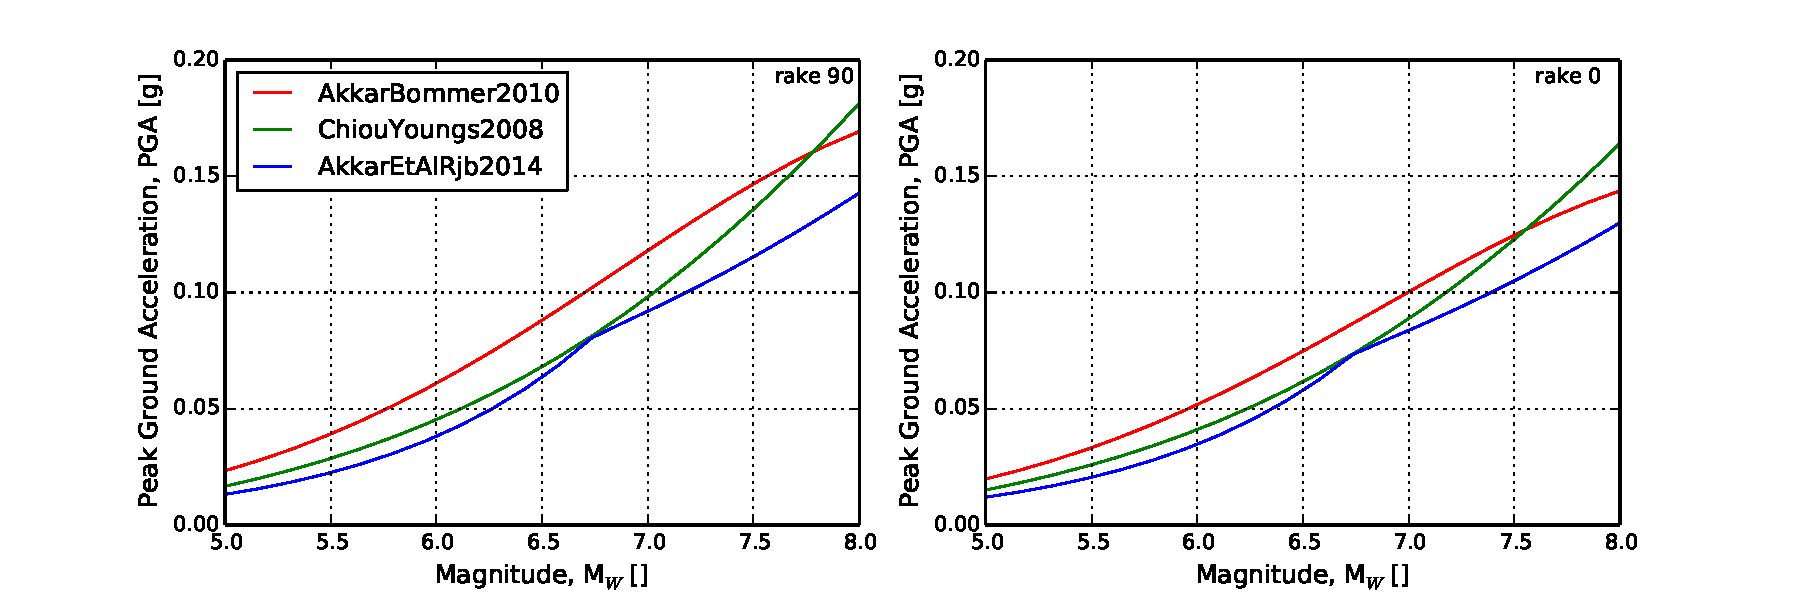
\includegraphics[trim = 23mm 0mm 23mm 5mm, clip, width=\textwidth]
    {./Pictures/gsim/mag_scaling_example.pdf}
\caption{Scaling of Peak Ground Acceleration as a function of magnitude 
    obtained by some of the \gls{acr:gsim} implemented in the \gls{acr:oqe}. 
    The ipython notebook used to generate this figure can be downloaded  
    \href{https://github.com/GEMScienceTools/hazard_book_2014/tree/lts/notebooks}{here}.}
\label{fig:gsim_mag_scaling}
\end{figure}
% . . . . . . . . . . . . . . . . . . . . . . . . . . . . . . . . . . . < Figure
%
\subsubsection{Distance}
\index{Ground-motion prediction equation!predictor variables!Source-site 
distance}
%
The OpenQuake-engine supports almost all the rupture-site 
distance metrics used by the most recent and complex 
\glspl{groundshakingintensitymodel} published in the scientific 
literature (see \ref{tab:distances} for a comprehensive list).
% --------------------------------------------------------------------->>> Table
\begin{table}[!t]
\centering
\begin{tabular}{|p{4.5cm}cp{7.5cm}|}
\hline
\rowcolor{anti-flashwhite}
\bf{Distance definition} & \bf{Symbol} & \bf{Description} \\
\hline 
Epicentral & R$_{epi}$ & Distance between the epicenter and the site. 
                         Note that currently in the \gls{acr:oqe} the 
                         hypocenter is assumed to be at the center of 
                         a rupture.\\
Hypocentral & R$_{hypo}$ & Distance between the hypocenter and the site. 
                           Note that currently in the \gls{acr:oqe} the 
                           hypocenter is assumed to be at the center of 
                           a rupture.\\
Joyner and Boore distance & R$_{jb}$ & Closest distance between the site and 
                                       the surface projection of the rupture \\
Closest distance to the rupture & R$_{rup}$ & Closest distance between 
                                              the site and the rupture 
                                              surface \\
Horizontal top-edge distance & R$_{x}$ & Horizontal distance between the site 
                                         and the top edge of the rupture \\
Top-of-Rupture depth & Z$_{tor}$ & Depth to the top edge of the rupture \\
\hline
\end{tabular}
\caption{Rupture-site distances supported by the \gls{acr:oqe}.}
\label{tab:distances}
\end{table}
% ---------------------------------------------------------------------<<< Table
The calculation of distances within the hazard component of the \gls{acr:oqe} 
is performed by assuming a spherical earth with a radius of 6371.0 km. 

Since earthquakes are always modelled in the \gls{acr:oqe} as finite ruptures 
all rupture-site metrics are always computed instantaneously. For this reason
the engine does not contain conversion equations between different metrics
\parencite[e.g.][]{scherbaum2004}
%
\subsubsection{Rupture mechanism}
\index{Ground-motion prediction equation!Rupture mechanism}
Many \glspl{acr:gsim} compute ground-motion according to 
different categories identifying major rupturing mechanisms such as normal,
strike-slip or reverse.

In the \gls{acr:oqe} the rupture mechanism of a seismic source is specified 
in terms of the rake angle (defined according to \cite{aki2002}). 
%
Since the rake is not used directly as a predictor variable in 
\glspl{acr:gsim}, most of the \gls{acr:oqe} implementations contain a mapping
between the rake angle and the rupture mechanism classes supported by each
specific model (see \cite[page 24 of][]{akkar2013r} for a review).
%
\subsubsection{Time averaged shear-wave velocity in the uppermost 30m 
(V$_{S,30}$)}
\index{Ground-motion prediction equation!Rupture mechanism! Time averaged
shear-wave velocity in the uppermost 30m, V$_{S,30}$}
%
Local soil conditions and their effects on the ground-motion are routinely 
incorporated into \glspl{groundshakingintensitymodel} by means of a scalar
quantity corresponding to the time-averaged shear wave velocity measured 
in the uppermost 30m of the soil column (V$_{S,30}$).
%
Local soil conditions in the \gls{acr:oqe} are specified by means of this
parameter.

In case of \glspl{groundshakingintensitymodel} which support the definition 
of local soil conditions through soil classes (e.g. hard rock, soft soil) 
their implementation is done in a way that given a value of V$_{S,30}$ the
corresponding soil class is used to compute the value of ground motion 
(provided that a mapping between soil classes and V$_{S,30}$ is defined 
by the authors).

Additional parameters used to quantitatively describe local geology are 
the depths to the 1 km/s and 2.5 km/s shear-wave velocity interfaces. 
These are parameters used in some \glspl{acr:gsim} (e.g. \cite{chiou2008}) 
to quantify the overall thickness of the soil column. 
%
\subsubsection{Depth to the top-of-rupture (Z$_{tor}$)}
\index{Ground-motion prediction equation!Rupture mechanism!Depth to the top of
rupture}
The depth to the top of rupture is a parameter introduced in some of the NGA
West 1 \gls{acr:gsim} such as \textcite{chiou2008} and \textcite{abrahamson2008}
following a supposed dependence of ground-motion to the depth of the source,
as suggested by \textcite{somerville2006a}.
%
% . . . . . . . . . . . . . . . . . . . . . . . . . . . . . . . . . . . . . . .
\subsection{Supported intensity measure types}
Each \gls{acr:gsim} implemented in the \gls{acr:oqe} provides a list of the 
supported \glspl{acr:imt}. Table \ref{tab:imts} contains a comprehensive list 
of possible options.
% --------------------------------------------------------------------->>> Table
\begin{table}[!h]
\centering
\begin{tabular}{|p{3cm}p{5cm}p{3cm}|}
\hline
\rowcolor{anti-flashwhite}
\bf{Acronym} & \bf{Description} & \bf{Unit of measure} \\
\hline 
PGA & Peak Ground Acceleration & g \\
PGV & Peak Ground Velocity     & cm/s \\
PGD & Peak Ground Displacement & \\
SA  & Spectral Acceleration    & g \\
IA  & Arias intensity &  \\
CAV & Cumulative Absolute Velocity &  \\
RSD & Relative Significative Duration \parencite{trifunac1975}&  \\
MMI & Modified Mercalli Intensity &  \\
\hline
\end{tabular}
\caption{Principal intensity measure types supported.}
\label{tab:imts}
\end{table}
% ---------------------------------------------------------------------<<< Table
The definitions of the ground-motion component supported are instead listed in
Table \ref{tab:hor_comp}. 
% --------------------------------------------------------------------->>> Table
% --------------------------------------------------------------------->>> Table
\begin{table}[!h]
\centering
\begin{tabular}{|p{6cm}p{7cm}|}
\hline
\rowcolor{anti-flashwhite}
\bf{Component} & \bf{Description} \\
\hline 
HORIZONTAL & General horizontal component \\
GEOMETRIC\_MEAN &  \\
%MEDIAN\_HORIZONTAL & Median of the two horizontal components \\
%AVERAGE\_HORIZONTAL & Median of the two horizontal components \\
GMRotI50 & Median value of the (period independent) geometric mean 
           \parencite{boore2006} \\
RotD50 & Median value of the (period dependent) geometric mean 
         \parencite{boore2010} \\
RANDOM\_HORIZONTAL & Random horizontal component \\
%GREATER\_OF\_TWO\_HORIZONTAL & Largest horizontal component of ground-motion \\
VERTICAL & Vertical component of ground-motion\\
\hline
\end{tabular}
\caption{Principal ground-motion components supported (THE CONTENT OF THIS 
TABLE MUST BE COMPLETELY REVISED)}
\label{tab:hor_comp} 
\end{table}
% ---------------------------------------------------------------------<<< Table

% ---------------------------------------------------------------------<<< Table
